% DAFN23 - Robotics - Lecture 3
% Roberto Masocco <roberto.masocco@uniroma2.it>
% May 24, 2023

\documentclass[aspectratio=169]{beamer}

% Slides layout
\usepackage[
    title={ROS 2},
    subtitle={Advanced communication},
    event={DAFN},
    author={Roberto Masocco},
    longauthor={Roberto Masocco},
    email={roberto.masocco@uniroma2.it},
    institute={Tor Vergata},
    longinstitute={University of Rome Tor Vergata},
    department={Department of Civil Engineering and Computer Science Engineering},
    researchgroup={},
    date={May 24, 2023}
]{utvengbeamer}

% Code listings settings
\usepackage[nomath]{lmodern}
\definecolor{codegreen}{rgb}{0 0.5 0}
\definecolor{codered}{rgb}{1 0 0}
\definecolor{codeocher}{rgb}{0.8 0.47 0.13}
\usepackage{listings}
\lstdefinestyle{beamer}{
    basicstyle=\ttfamily\small,
    commentstyle=\color{codegreen},
    breakatwhitespace=false,
    captionpos=b,
    frame=lines,
    keepspaces=true,
    keywordstyle=\color{codered}\bfseries,
    numbers=left,
    numbersep=5pt,
    numberstyle=\footnotesize,
    showspaces=false,
    showstringspaces=false,
    showtabs=false,
    stringstyle=\color{codeocher},
    tabsize=2
}
\lstset{style=beamer}
\lstdefinelanguage{ros2msg}{
  alsoletter={[, ], _, /},
  morecomment=[l][\color{codegreen}]{\#},
  morekeywords={int64, uint32, string, uint8, uint8[], int32, int32[], std_msgs/Header}
}

\usepackage{hyperref}
\usepackage{wasysym}

\begin{document}

% --- Title page ---
\frame{\titlepage}

% --- Recap ---
% Recap
% Roberto Masocco <roberto.masocco@uniroma2.it>
% May 16, 2024

% --- Recap ---
\begin{frame}{Recap}
\textbg{Messages} are the most basic, \textbg{one-way} communication paradigm.\\
\bigskip
\textbg{QoS policies} and other topic settings affect communication behavior among entities.\\
\bigskip
\textbg{Services} are a simple implementation of a \textbg{two-way}, \textbg{client-server} communication paradigm.\\
\bigskip
This lecture is \href{https://github.com/robmasocco/DAFN24_Robotics_4}{\color{blue}\underline{here}}.
\end{frame}
\begin{frame}{Recap}
  \begin{block}{Updates}
    \begin{itemize}
      \item \textbf{Updated code examples}, please pull new commits!
      \item Follow-up on \textbf{message topics code examples}:
      \begin{itemize}
        \item \href{https://github.com/IntelligentSystemsLabUTV/ros2-examples/blob/humble/src/cpp/topic_pubsub_cpp/src/resetting_sub.cpp}{\color{blue}\underline{\texttt{resetting\_sub}}} example.
      \end{itemize}
    \end{itemize}
  \end{block}
\end{frame}


% --- Table of contents ---
\begin{frame}
	\frametitle{Roadmap}
	\tableofcontents
\end{frame}

% --- Section 1 ---
% Section 1 - Asynchronous I/O
% Roberto Masocco <roberto.masocco@uniroma2.it>
% May 24, 2023

% ### Asynchronous I/O ###
\section{Asynchronous I/O}
\graphicspath{{figs/section1/}}

% --- What is I/O? ---
\begin{frame}{What is I/O?}{Informal definition}
  In an \textbg{operating system}, a \textbg{task} (specifically, a \textbg{thread}) can perform operations pertaining to these two broad families:
  \begin{itemize}
    \item execute \textbg{computations} (\emph{e.g.}, \texttt{1 + 1 = 2}), using regular \textbg{CPU} instructions;
    \item access \textbg{system resources} (both \textbg{hardware} and \textbg{software}) through calls to the \textbg{kernel} (\emph{i.e.}, \textbg{system calls}), \textbg{exchanging data} in both directions.
  \end{itemize}
  When these resources are not part of the OS, but rather the OS enables tasks to interface\footnote{Drivers, protocols, software stacks...} with them, we talk about \textbg{I/O} (\emph{Input/Output}).
  \newline\newline
  OS schedulers typically distinguish between \textbg{CPU-bound} and \textbg{I/O-bound} tasks, because of their different \textbg{execution patterns}.
\end{frame}

% --- Blocking I/O ---
\begin{frame}{Blocking I/O}{What the OS likes the most}
  The most common execution pattern for a task that performs an I/O system call goes like this:
  \begin{enumerate}
    \item prepare the \textbg{input data} for the system call;
    \item call an \textbg{API} that performs the system call;
    \item the OS \textbg{blocks the task}, which is \textbg{waiting} for the operations to complete;
    \item the OS \textbg{returns control} to the task when the system call is completed;
    \item \textbg{output data}, returned by the kernel, can be accessed by the task.
  \end{enumerate}
  This is \textbg{blocking I/O}, because the task is \textbg{blocked} while waiting for the system call to complete.
  \newline\newline
  Examples of \textbg{blocking calls}: \texttt{read}, \texttt{write} to \textbg{file descriptors}.
\end{frame}

% --- Non-blocking I/O ---
\begin{frame}{Non-blocking I/O}{What userspace application like the most}
  If the kernel supports this feature, a task can perform a \textbg{non-blocking system call}:
  \begin{enumerate}
    \item prepare the \textbg{input data} for the system call;
    \item call an \textbg{API} that performs the system call;
    \item the OS \textbg{returns control} to the task \textbg{immediately}, without blocking it;
    \item the task can \textbg{poll} the system call \textbg{status} to check if it is completed;
    \item when the system call is completed, the task can \textbg{access the output data};
    \item optionally, a \textbg{callback} routine can be registered to be executed right when the system call is completed.
  \end{enumerate}
  This is \textbg{non-blocking I/O} (or \emph{asynchronous I/O}, or \emph{overlapped I/O}), because the task is \textbg{not blocked} while waiting for the system call to complete, and things can happen in between.
  \newline\newline
  Examples of \textbg{non-blocking calls}: \texttt{read}, \texttt{write} to \textbg{sockets} configured appropriately.
\end{frame}
\begin{frame}{Non-blocking I/O}{What userspace application like the most}
  Usually, the operation status can be inspected through some kind of \textbg{handle object} returned by the API.
  \newline\newline
  Some \textbg{programming languages} implement \textbg{future objects}: datatypes that hold the result of an asynchronous operation, which can be inspected to check if the operation is completed, and to retrieve the result once it is; \textbg{they are said to hold a value only when the operation is completed}.
  \begin{alertblock}{}
    \centering
    \textbr{ROS 2} makes a heavy use of \textbr{callbacks} and \textbr{future objects} to handle \textbr{asynchronous I/O}.
  \end{alertblock}
\end{frame}


% --- Section 2 ---
% Section 2 - Services
% Roberto Masocco <roberto.masocco@uniroma2.it>
% May 24, 2023

% ### Services ###
\section{Services}
\graphicspath{{figs/section2/}}

% --- ROS 2 services ---
\begin{frame}{ROS 2 services}{Basic client-server paradigm}
  ROS 2 extends the basic DDS messages adding two more \textbg{communication paradigms}: the first is the \textbg{service}. It allows nodes to establish quick and simple \textbg{client-server} communications.
  \begin{figure}
    \centering
    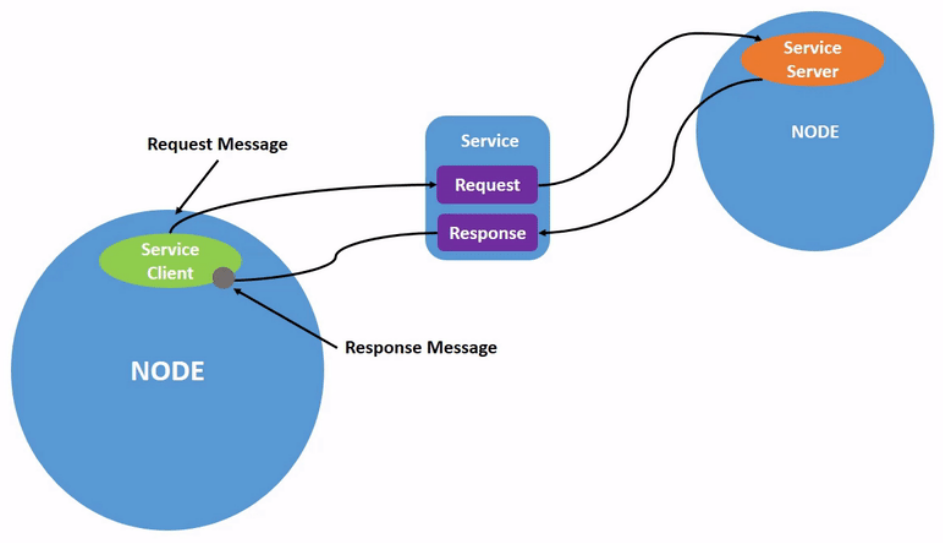
\includegraphics[scale=.33]{ros2Srv.png}
    \caption{Two nodes acting as service \emph{client} and \emph{server}.}
    \label{fig:ros2srv}
  \end{figure}
\end{frame}
\begin{frame}{ROS 2 services}{Communication overview}
  In actual ROS 2 applications:
  \begin{enumerate}
    \item The \textbg{client} sends a \textbg{request message} to the server.
    \item The \textbg{server} receives the request and processes it.
    \item Meanwhile, the \textbg{client} can either \textbg{block} waiting for the response or \textbg{synchronously poll} it.
    \item When done, the \textbg{server} sends a \textbg{response message} to the client.
    \item If waiting, the \textbg{client} awakes when receiving the response.
  \end{enumerate}
\end{frame}
\begin{frame}{ROS 2 services}{CLI introspection tools}
  The main command is \texttt{ros2 service} with the following verbs:
  \begin{itemize}
    \item \texttt{list} Lists all active services.
    \item \texttt{type} Prints the service type.
    \item \texttt{find} Lists active services of the given type.
    \item \texttt{call} Calls the service with the request defined in the command line.
  \end{itemize}
\end{frame}
\begin{frame}{ROS 2 services}{Coding hints for servers and clients}
  \begin{block}{Servers}
    Similarly to topic subscriptions, requests are processed in appropriate \textbf{callbacks}, taking \textbf{two arguments}, in which responses are also populated. The server object is as well only needed to instantiate the service.
  \end{block}
  \begin{block}{Clients}
    As per the previous dynamics, one has to \textbf{code each step} of the client side into their application using appropriate \textbf{ROS 2 APIs}. \textbf{The client object is used to send requests}, while \textbf{responses are handled as \texttt{future} objects\footnote{\href{https://en.cppreference.com/w/cpp/thread/future}{\color{blue}\underline{\texttt{std::future} - C++ Reference}}}}.
  \end{block}
\end{frame}

% --- Interface files - Services ---
\begin{frame}[fragile]{Interface files}{Services}
  The entire system is built on messages, so \textbg{combine two of them} in a single interface file, separated by \texttt{-{}-{}-}.\\
  Service file names end with \texttt{.srv}.
  \begin{columns}
  \column{.9\textwidth}
  % Listing: example_interfaces/srv/AddTwoInts service definition
  \begin{lstlisting}[language=ros2msg, caption=Definition of the \texttt{example\_interfaces/srv/AddTwoInts} service.]
# REQUEST
int64 a
int64 b
---
# RESPONSE
int64 sum\end{lstlisting}
  \end{columns}
\end{frame}

% --- Example - Simple service ---
\begin{frame}{Example}{Simple service}
  \begin{block}{}
    \centering
    Now go have a look at the \href{https://github.com/IntelligentSystemsLabUTV/ros2-examples/tree/humble/src/cpp/simple_service_cpp}{\color{blue}\underline{\texttt{ros2-examples/src/cpp/simple\_service\_cpp}}} package!
  \end{block}
\end{frame}


% --- Section 3 ---
% Section 3 - Actions
% Roberto Masocco <roberto.masocco@uniroma2.it>
% May 24, 2023

% ### Actions ###
\section{Actions}
\graphicspath{{figs/section3/}}

% --- Limitations of services ---
\begin{frame}{Limitations of services}
  The third paradigm exists because services rely on the following \textbg{restrictive assumptions}.
  \begin{alertblock}{Services implementation assumptions}
    \begin{itemize}
      \item Since the client may block for the entire duration of the request processing, \textbr{server computations should be short and always produce some result} (\emph{e.g.}, even an error must be a result, but \textbr{we} have to encode it).
      \item Service calls are finished only when the response has been received, \emph{i.e.}, \textbr{if either the client or the server crash, the behaviour of the other one is undefined} (no \textbr{state machine}! Say hello to \textbr{deadlocks}, crashes...).
      \item Once a service is called, \textbr{the request may never be interrupted}.
    \end{itemize}
  \end{alertblock}
  These make operations that \textbg{must be requested} and \textbg{take a long time} (for CPUs!) completely unfeasible.\\
  Think of real stuff such as \textbg{movement}, \textbg{navigation}...
\end{frame}

% --- ROS 2 actions ---
\begin{frame}{ROS 2 actions}{Full client-server paradigm}
  Built on services and message topics, they \textbg{decouple computations from middleware APIs}, thanks to three concepts that embody the \textbg{three stages of the communication}:
  \begin{enumerate}
    \item \textbg{Goal}: the full request of the operation to be executed.
    \item \textbg{Feedback}: intermediate results and information about the ongoing processing.
    \item \textbg{Result}: the final result of the requested operation.
  \end{enumerate}
  \vspace{.5cm}
  Their implementation is still a bit cumbersome because of the \textbg{many different data types} (classes) involved, and is found in the \href{https://github.com/ros2/rclcpp/tree/humble/rclcpp_action}{\color{blue}{\underline{\texttt{rclcpp\_action}}}} and \href{https://github.com/ros2/rclpy/tree/humble/rclpy/rclpy/action}{\color{blue}{\underline{\texttt{rclpy action}}}} libraries.
  \newline\newline
  They are \textbg{extensively used for robot navigation and movement}.
\end{frame}
\begin{frame}{ROS 2 actions}{Full client-server paradigm}
  \begin{figure}
    \centering
    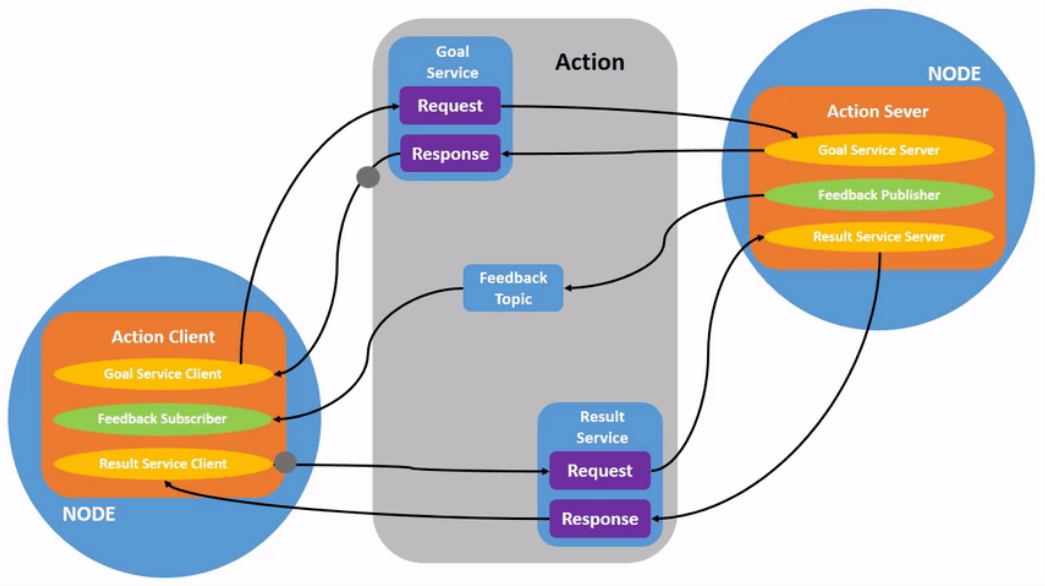
\includegraphics[scale=.37]{ros2Act.png}
    \caption{Example of an action \emph{server} and \emph{client}.}
    \label{fig:ros2Act}
  \end{figure}
\end{frame}
\begin{frame}{ROS 2 actions}{The goal state machine}
  \begin{figure}
    \centering
    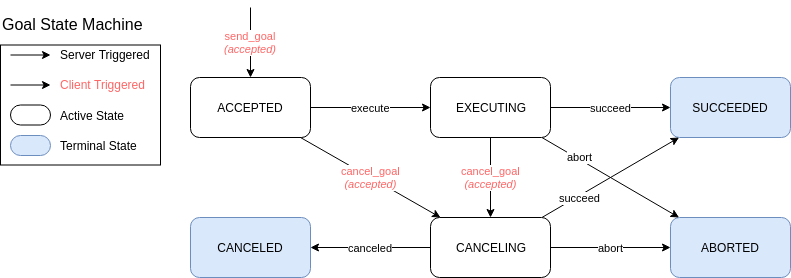
\includegraphics[width=\textwidth]{goalStateMachine.png}
    \caption{State machine\footnote{\href{http://design.ros2.org/articles/actions.html}{\color{blue}\underline{Actions - ROS 2 Design}}} of an action goal, implemented and managed internally by ROS 2.}
    \label{fig:goalStateMachine}
  \end{figure}
\end{frame}
\begin{frame}{ROS 2 actions}{Communication overview}
  In actual ROS 2 applications, the \textbg{client} requests the completion of some \textbg{goal} to the \textbg{server}. The middleware only offers APIs to \textbg{notify the state of the goal} between the two.
  \begin{enumerate}
    \item The \textbg{client} sends a \textbg{goal service request} to the server.
    \item The \textbg{server} may \textbg{accept} or \textbg{reject} the goal request.
    \item Server computations are usually started when the goal is \textbg{executed}: the middleware only keeps track the state of the goal, its updates and the rest are up to the developer.
    \item The \textbg{client may cancel} the goal request; the \textbg{server may abort} the goal request; intermediate results and information, if any, are published by the server on the \textbg{feedback topic}.
    \item The \textbg{client} asks the server for the final result over the \textbg{result service}.
  \end{enumerate}
\end{frame}
\begin{frame}{ROS 2 actions}{CLI introspection tools}
  The main command is \texttt{ros2 action} with the following verbs:
  \begin{itemize}
    \item \texttt{list} Lists all active actions.
    \item \texttt{info} Prints information about an action.
    \item \texttt{send\_goal} Sends a goal request to an action server, and prints the result; with \texttt{-f} prints also feedback messages.
  \end{itemize}
\end{frame}
\begin{frame}{ROS 2 actions}{Coding hints for servers and clients}
  \begin{block}{Servers}
    Goal requests are handled with \textbf{callbacks}, while computations can be handled freely (usually in \textbf{separate threads}). When done, the goal must be marked as \textbf{succeeded} or \textbf{aborted}.
  \end{block}
  \begin{block}{Clients}
    Similarly to services, much is done with \textbf{\texttt{future} objects}, but \textbf{callbacks} must be defined to handle \textbf{goal}, \textbf{result} and \textbf{cancellation responses}, and \textbf{feedbacks}.
  \end{block}
  \begin{block}{}
    \centering
    Handling all possible scenarios for a goal results in the \textbf{longest and most complicated code that a ROS 2 application may ever require}. {\Large\smiley{}}
  \end{block}
\end{frame}

% --- Interface files - Actions ---
\begin{frame}[fragile]{Interface files}{Actions}
  Combine \textbg{three messages} in a single interface file, separated by \texttt{-{}-{}-}.\\
  Action file names end with \texttt{.action}.
  \begin{columns}
  \column{.9\textwidth}
  % Listing: ros2_examples_interfaces/action/Fibonacci action definition
  \begin{lstlisting}[language=ros2msg, caption=Definition of the \texttt{ros2\_examples\_interfaces/action/Fibonacci} action.]
# GOAL
int32 order
---
# RESULT
int32[] sequence
---
# FEEDBACK
int32[] partial_sequence\end{lstlisting}
  \end{columns}
\end{frame}

% --- Example - Fibonacci computer ---
\begin{frame}{Example}{Fibonacci computer}
  \begin{block}{}
    \centering
    Now go have a look at the \href{https://github.com/IntelligentSystemsLabUTV/ros2-examples/tree/humble/src/cpp/actions_example_cpp}{\color{blue}\underline{\texttt{ros2-examples/src/cpp/actions\_example\_cpp}}} package!
  \end{block}
  If you're curious, the \href{https://github.com/IntelligentSystemsLabUTV/ros2-examples/tree/humble/src/cpp/advanced/complete_actions_cpp}{\color{blue}\underline{\texttt{ros2-examples/src/cpp/advanced/complete\_actions\_cpp}}} package, which implements the complete goal state machine using a multithreaded executor.
\end{frame}


% --- Exercises ---
\begin{frame}{Exercises}
	\begin{itemize}
		\item Run the action client and server examples, and try to call the action from the command line.
		\item Modify the feedback message: instead of a partial sequence, it should publish the length of the sequence so far; this requires:
		      \begin{enumerate}
			      \item modifying the action definition in \texttt{ros2\_examples\_interfaces};
			      \item modifying the server node to publish the length of the sequence instead of the partial sequence in the feedback message (hint: use methods of the \texttt{std::vector} class to get the length of the partial sequence in one go);
			      \item modifying the feedback callback in the client to parse and print the length from the feedback message.
		      \end{enumerate}
	\end{itemize}
\end{frame}

\end{document}
